% vim: set foldmethod=marker :

% Villancico book chapter on Zaragoza

% 2013-02-08 v0 
% 2013-07-01 v1 
% 2014-12-15 v2 	Caseda section based on revision for ACLS, 2013-09
% 2014-12-29 v2.1 	Real revision
% 2015-03               Dissertation defended
% 2019-04-18            Imported for monograph
% 2019-05-28            Monograph revision begun
% 2019-06-25            Good enough for now!
% 2020-02-10            Final revisions

\chapter{Offering and Imitation (Zaragoza, 1650--1700)}
\label{ch:zaragoza}

\epigraph
{No son a los sentidos \\
lo que suenan sus voces soberanas \\
porque de este instrumento \\
cuantas ellos percibían serán falsas.}
{Vicente Sánchez, \wtitle{Con dulces accentos} (Zaragoza, 1688)}

%{{{1 intro
As composers like Gutiérrez de Padilla and Cererols were imitating heavenly
harmony in their music, they were also imitating earthly models in a tradition
of metamusical composition.
Their acts of imitation were also acts of offering.
In human terms, they offered a tribute to mentors and contributed to a peer
community.
In the religious sense, this devotional music was an act of offering to God,
through which listeners were given the opportunity to offer themselves.

\index{Gutiérrez de Padilla, Juan}
\index{Cererols, Joan}

This chapter focuses on the changing nature of imitation within a network of
composers in the province of Zaragoza.
We have already seen that Zaragoza was a principal node in the network of
villancico composers and poets.
The first case study in this chapter examines two successive settings of the
same textual family by Pablo Bruna and Miguel Ambiela.
This is a clear case of a younger composer imitating the work of a respected
musician of the preceding generation---not only using the same words but
adapting some of the same musical ideas as well.

\index{Zaragoza}
\index{networks}
\index{Bruna, Pablo}
\index{Ambiela, Miguel}
\index{imitation}
\index{homage}

The final section discusses the villancico \wtitle{Qué música divina} by José
de Cáseda of Zaragoza, preserved in a convent collection from Puebla, in which
the conventions of the metamusical villancico tradition are pushed to a
particular extreme.
The increasing weight of convention in this type of music required composers to
devise ever-new ways to represent the relationship between heavenly and earthly
music.
The piece compares Christ to a \term{vihuela}, and imitates this plucked-string
instrument by effectively turning the vocal ensemble into a vihuela.
The three villancicos studied in this chapter present music as an affective
devotional practice of self-offering, in keeping with their ritual functions
for Eucharistic and Marian devotion.

\index{Cáseda, José de}
\index{musical instruments, symbolism}
\index{\emph{vihuela}}
\index{villancico!liturgical function!Eucharistic devotion}
\index{villancico!liturgical function!sanctoral devotion}

%}}}1

%{{{1 Bruna vs Ambiela
\section{\quoted{Let Voices Ascend to Heaven}: From Bruna to Ambiela}

%{{{2 background
Zaragoza was an important religious center in the crown of Aragon, with its two
principal churches, the cathedral of La Seo and the basilica of El Pilar (today
co-cathedrals).%
    \Autocite{Ezquerro:CatalogoZaragoza}
A large proportion of the surviving villancico poetry imprints were published
in Zaragoza, many of them commemorating performances of music by Diego de
Cáseda or his son José.
In the greater province of Zaragoza, the village of Daroca was home to the
acclaimed organist Pablo Bruna.  
Miguel Ambiela, from the same province, received his early training in Daroca
before graduating to highly prestigious posts in Zaragoza, Madrid, and Toledo.

\index{Zaragoza!La Seo}
\index{Zaragoza!El Pilar}
\index{Bruna, Pablo|(}

The first known version of \wtitle{Suban las voces al cielo} is a Eucharistic
villancico composed by Pablo Bruna for four voices (SSAT) with accompaniment,
preserved in the archive of Girona Cathedral.%
    \Autocites
    [29--34 (no archival signature given)]{Calahorra:DarocaEdition}
In 1986 Pedro Calahorra identified the relationship between it and a 
villancico with the same incipit by Miguel Ambiela.%
\begin{Footnote}
    \sig{E-Bbc}{M/733/1}; 
    \autocites
    {Calahorra:Suban}
    [35--45]{Calahorra:DarocaEdition}.
\end{Footnote}
He called Ambiela's work a \quoted{parody villancico}, \quoted{an homage from a
pupil to his teacher}.%
    \Autocite[9]{Calahorra:Suban}
But there is more to the relationship than Calahorra's brief analysis could
explore, and the differences between the pieces are as significant as the
similarities.
Moreover, a new, previously unattributed, source of the Bruna villancico
provides further insight into this work.%
    \footnote{\sig{E-Bbc}{M/759/44}.}

\index{Girona!Cathedral}
\index{Gerona|see{Girona}}
\index{homage}
\index{villancico!sources}
\index{Barcelona}
%}}}2

%{{{2 Bruna
\subsection{Bruna: Voices as Flames of Self-Offering}

Born in 1611 in Daroca, Bruna served as organist at the collegiate church of
Santa María de los Sagrados Corporales from 1631 until his death in 1679.% 
    \Autocite[104]{Calahorra:Aragon}
His musicianship, which was not hindered by being blind from an early age, was
renowned throughout the region.
In 1639 he was offered the organist position at El Pilar in Zaragoza but
declined it.% 
    \Autocite[123--125]{Calahorra:Aragon}
Bruna's organ music was disseminated more widely through its inclusion in the
anthology \wtitle{Huerto ameno de varias flores de música} collected by Fray
Antonio Martín y Coll and published in Madrid in 1709.

\index{Martín y Coll, Antonio}
\index{Daroca!Santa María de los Sagrados Corporales}
\index{Zaragoza!El Pilar}

Bruna's villancico would function well for Eucharistic devotion, in both its
poetic content and musical style.  
The piece fits a subtype of chamber villancico dedicated \foreign{al Santísimo
Sacramento} (to the Blessed Sacrament) and intended not for the triumphalistic 
public festivities of Corpus Christi, but for more reflective occasions of
Eucharistic adoration.
This more intimate type of Eucharistic villancico frequently features
mystically-infused texts with an emphasis on personal affective devotion to
Christ in the sacrament.  
Bruna's madrigalesque counterpoint for four voices is similar to other such
pieces from before 1660, in contrast to the solo and duo continuo-songs that
predominate later.%
\begin{Footnote}
    The Girona manuscript does include an accompaniment part labeled
    \foreign{entablatura}, but this is primarily a \term{basso seguente} rather
    than the independent continuo part found in Irízar and Carrión.
\end{Footnote}

\index{villancico!liturgical function!Eucharistic devotion}
\index{villancico!dedications!\emph{al Santísimo Sacramento}}

The central image in Bruna's villancico is the soul as a burning phoenix,
consumed by the love of God.
This use of fire symbolism may be found in other Eucharistic villancicos, such
as a 1643 piece by Jaume Pexa from Lleida (Lérida)
(\poemref{poem:Que_me_quemo-Pexa}), with an estribillo similar to Bruna's.%
\begin{Footnote}
    \sig{E-Bbc}{M/765/15}; see \shortcite[\sv{Pexa, Jaume}]{DMEH}.
    The manuscript is in the same box of villancicos as the Barcelona version
    of Cererols's \wtitle{Suspended, cielos}, as well as a piece by Miguel
    Ambiela and another by one of the Cásedas (probably Diego, the elder).  
\end{Footnote}
The partbooks of Pexa's eight-voice piece bear the heading \foreign{De amores
del exposo sancto} (About love for the exposed Sacrament), making clear that
the piece was to be performed for Eucharistic adoration.  

\index{fire}
\index{phoenix}
\index{love}
\index{Pexa, Jaume}
\index{Lleida}
\index{Lérida|see{Lleida}}

%{{{4 poem pexa
\begin{poemexample}
    \caption{\wtitle{Que me quemo}, villancico for Eucharistic adoration by
    Jaume Pexa (Lleida, 1643), estribillo}
    \label{poem:Que_me_quemo-Pexa}
    \includefloat{Que_me_quemo-Pexa}
\end{poemexample}
%}}}4

The anonymous poet of Bruna's villancico combines the conceit of the soul as a
burning phoenix with a musical conceit announced in the first line: \quoted{Let
voices to ascend to heaven} (\poemref{poem:Suban_las_voces-Bruna-estribillo},
\ref{poem:Suban_las_voces-Bruna-coplas}).
As a poem, the estribillo of \wtitle{Suban las voces} may be divided into three
sections. 
First, the opening quatrain in \term{romance} (\poemlines{1--4}) establishes
the primary conceit linking the voice and the phoenix.
The next section switches to seven-syllable \term{romancillo}
(\poemlines{5--11}) and, rather like \term{Voces, las de la capilla}, presents
a scene of music-making using technical keywords.
The estribillo closes with a couplet (\poemlines{12--13}) that epitomizes the
conceit: \quoted{a soul that burns}.
Lines 4 and 13, both truncated to five syllables, mark ending points in the
text, while assonance throughout unifies the poem.

\index{poetic meter}

%{{{4 poem bruna
\begin{poemexample}
    \caption{\wtitle{Suban las voces al cielo}, setting I, poetic text set by
    Bruna, estribillo}
    \label{poem:Suban_las_voces-Bruna-estribillo}
    \includefloat{Suban_las_voces-Bruna-estribillo}
\end{poemexample}

\begin{poemexample}
    \caption{\wtitle{Suban las voces}, setting I, poetic text set by Bruna,
    coplas} 
    \label{poem:Suban_las_voces-Bruna-coplas}
    \includefloat{Suban_las_voces-Bruna-coplas}
\end{poemexample}
%}}}4

The coplas differ between the Girona and Barcelona manuscripts.
The first copla is identical in both sources, but the Girona version follows it
with two stanzas, while the Barcelona version follows it with five unique
stanzas.
The Barcelona coplas all follow the same metrical scheme as copla 1: three
octosyllablic lines and the refrain \foreign{arde}, with \emph{a/e} assonance
in the even lines.
The Girona coplas, by contrast, change the metrical pattern after copla 1: they
add an additional line and maintain assonance only in the last syllables; the
\foreign{arde} refrain no longer forms part of the metrical structure.
These differences suggest that the Barcelona coplas are closer to the original
source of this textual family, while the different Girona coplas were likely
penned by a later poet, possibly to replace verses that had been lost or
forgotten.
The theology and tone of the texts also suggests that the Barcelona source is
older, as the Girona coplas are slightly more didactic.
This recalls the way later versions in the \wtitle{Voces, las de la
capilla} and \wtitle{Suspended, cielos} families simplified and explained their
models (\chapref{ch:padilla-voces}, \ref{ch:cererols-suspended}).

Similar to Juan Gutiérrez de Padilla, Bruna projects each phrase of poetic
text through a distinct phrase of music, with its own rhythmic and harmonic
profile, and closely follows the natural stresses of the words.  
The three poetic sections are also clearly articulated in the musical form
through shifts of meter and character.
Bruna also has his musicians depict the musical concepts in the poem in a
madrigalistic manner.  
The singers perform \quoted{let voices ascend} by leaping upward on
\foreign{voces} and then repeating the whole phrase again a third higher---a
musical-rhetorical \term{anaphora}, since the term means both repeating a
phrase and \quoted{lifting up}.
Bruna follows the first section with a change of meter (to \meterC), and his
setting of \foreign{Y mudando el aire en veloces corcheas} uses appropriately
flying \foreign{corcheas} (eighth notes), ascending and descending in pairs
(\foreign{juntas}) (\musref{mus:Bruna-Suban_las_voces-estribillo}).
Bruna sets \foreign{en síncopas que elevan} exactly as would be expected, with
syncopated phrases that leap upwards like flames.
Bruna uses chromatic alterations for the phrase \foreign{bemoles blandos},
writing E flats in the outer voices and then setting up a
striking Phrygian cadence in in which the Alto leaps upwards
into an unprepared seventh.  
Bruna writes dotted figures on \foreign{trinados que suspendan} that flow into
textbook suspensions; the dotted gestures would invite any singer to add a
trill.
For \foreign{digan en paso} (let them say in turn) Bruna has the voices follow
each other in fugal imitation, in an evenly paced rhythmic pattern.

\index{text depiction}

%{{{4 music Bruna estribillo
\begin{musicexample}
    \caption{Bruna, \wtitle{Suban las voces}, estribillo: Madrigalistic text
    setting (accompaniment omitted)}
    \label{mus:Bruna-Suban_las_voces-estribillo}
    \includefloat{Bruna-Suban_las_voces-estribillo}
\end{musicexample}
%}}}4

In the coplas Bruna breaks up the declamation-focused setting with a syncopated
rhythm on \foreign{si en Dios hallas nueva vida} (if you find new life in God):
by dividing three measures of duple time into what sounds like four measures of
triple, he animates this phrase with a new kind of rhythmic life. 
Similarly, in the ending refrain line on \foreign{arde}, Bruna syncopates the
rhythm by playing off the voices in pairs, where in each measure one group has
downbeat accents and the other has a minim rest followed by an offbeat accent.
These rests create a breathless intensity that fittingly portrays the soul in
ardor.

\index{rhythm}

This passage points to a more dramatic quality of Bruna's setting that goes
beyond text depiction to express a mystical affect, partly through the use of
chromaticism.
For example, in \measure{7}, the voice and accompaniment undulate between a
G-over-E\fl{} harmony and F\sh-over-D, on the words \quoted{a phoenix is
burning, a soul}.
These minor-second gestures and chromatic alterations may be
ways of depicting spiritual passion, and of creating a stylistic topic that
could incite heartfelt devotion.
Altered notes could symbolize the changes wrought by fire, which, as we will
explore below, is a metaphor for the soul's conversion to loving God.  

\index{text expression}
\index{affects}
\index{Bruna, Pablo|)}
%}}}2

%{{{2 Ambiela
\subsection{Ambiela: Voices Rising in Intercession}

%{{{3 background, sources
The later setting in this villancico was composed by Miguel Ambiela
(1666--1733) to a text closely based on that set by Bruna.
Where Bruna's piece concentrated on the symbolism of fire and the phoenix,
Ambiela's is dedicated to the Assumption of the Virgin Mary.
The compositor of the text---quite possibly Ambiela himself---has excerpted
from the earlier poem all the lines with musical vocabulary and built a new
poem around them focused on raising voices to celebrate Mary as heavenly
intercessor (\poemref{poem:Suban-2-estribillo}, \tabref{tab:Bruna-Ambiela-cf}).

\index{Ambiela, Miguel|(}
\index{villancico!dedications!Assumption of Mary}
\index{sanctoral devotion!Mary}

%{{{4 poem Suban Ambiela estribillo
\begin{poemexample}
    \caption{\wtitle{Suban las voces al cielo}, setting II by Miguel Ambiela,
    estribillo} 
    \label{poem:Suban-2-estribillo}
    \includefloat{Suban-2-estribillo}
\end{poemexample}
%}}}4

%{{{4 table Bruna Ambiela cf
\begin{table}
    \caption{\wtitle{Suban las voces}: Comparison of estribillos set by Bruna
    and Ambiela} 
    \label{tab:Bruna-Ambiela-cf}
    \includefloat{Bruna-Ambiela-cf}
\end{table}
%}}}4

Ambiela lived through the upheavals caused by the end of the Habsburg dynasty,
in a career that took him from the town of La Puebla de Albortón in Zaragoza
province to the most prestigious positions in Spain, as chapelmaster of El
Pilar in Zaragoza (1700--1707), Las Descalzas Reales in Madrid (1707--1710),
and finally Toledo Cathedral (1710--1733).%
    \Autocites
    [1]{Calahorra:Suban}
    [\sv{Ambiela}]{Grove}
    {Alvarez:Ambiela}
His training began at age 15, when in 1681 his parents sent him to study music
in Daroca.
Within four years Ambiela had been appointed chapelmaster at the collegiate
church there, where Bruna had been organist.
Since Bruna died in 1678, Ambiela likely did not study with him (as Calahorra
speculated), but he probably did encounter Bruna's music during his time in
Daroca, and may have even performed it.%
    \Autocite{Calahorra:Suban}
He could have encountered the piece in the church's archive during the year he
served as chapelmaster (1685--1686), before moving on to a position in Lleida.
Ambiela's version of \wtitle{Suban las voces} could have signalled to listeners
in the parish that their new chief musician was at once the heir to the
esteemed legacy of Bruna and a creative new voice of his own.

\index{teaching}
\index{apprenticeship}
\index{La Puebla de Albortón (Zaragoza)}
\index{Zaragoza!El Pilar}
\index{Madrid!Las Descalzas Reales}
\index{Toledo Cathedral}
\index{Daroca}
\index{Lleida}
\index{affiliation}

Supporting evidence that young Iberian composers modeled new music on older
works encountered in local archives comes from the surviving manuscript lesson
books from apprentice musicians.
One such notebook, written in Catalan, concludes with a section on \quoted{Some
Rules about Counterpoint Observed from the Method of Some Masters in Girona}.%
    \Autocite{Cpt-Notes-Girona}
A student has copied out a list of guidelines followed by a selection of
excerpts from pieces he encountered in the archive.

\index{education}
\index{imitation}

Ambiela's ambitious setting for six voices (SST, SAT, continuo) is preserved in
manuscript performing parts in Barcelona, copied sometime before 1689.%
\begin{Footnote}
    \sig{E-Bbc}{M/733/1}.
    Calahorra's edition misplaces one of the fugal entries: the Alto II that
    enters on \foreign{Vuelen, vuelen juntas} in \measure{22} of the edition
    should enter on the fourth semiminim of the \measure{23}.
\end{Footnote}
The front-facing leaf used as a title page bears a dedication to the Assumption
of Mary in one scribal hand, and a series of doodles on the name Torrente in a
second, sloppier hand---the work, it appears, of an idle-handed choirboy by
that name.
The same writer also copied his own \term{bajón} part and, at the top of the
accompaniment part, dated and ascribed the piece quite specifically:
\quoted{Acompañamiento Continuo a 6 Vozes del Maestro Miguel Ambiela año 1689 a
24 octobre}.
The 24th of October was the feast of St. Raphael, Archangel, but since the
villancico was clearly intended for the Assumption of the Virgin on August 15,
this date was either a later performance or just the copying date.
In 1689 the 23-year-old Ambiela was chapelmaster in Lleida, halfway between
Zaragoza and Barcelona.  
On the title leaf, the same hand (Torrente) credits the piece to \quoted{Master
Miguel Ambiela, who was from Lérida and before that from Daroca, where the wall
is big and the city is small}.%
\begin{Footnote}
    \sig{E-Bbc}{M/733/1}: \quoted{Del Maestro Miguel Ambiela/ que fue de
    Lerida y despues de daroca en donde el muro/ es Grande y la Ciutat es
    Poca}.
\end{Footnote}
The copyist, writing in Castilian, spells \foreign{ciudad} with the
Catalan-inflected phonetic spelling \foreign{ciutat},
just as in the Cererols manuscripts in the previous chapter,
\foreign{suspended} was copied \foreign{suspendet}.  
The trace of a Catalan accent, along with the joke disparaging Daroca---a small
town surrounded by huge medieval walls---both suggest that the writer was a
member of Ambiela's chapel in Lleida.
That young master Torrente highlights Ambiela's previous position in Daroca
suggests that, regional rivalry aside, there was some local significance in
Ambiela's connection to that city, likely because of the piece's connection to
Pablo Bruna.

\index{Catalonia}
\index{villancico!sources}
\index{performers!boys}
%}}}3

%{{{3 outdoing
\subsubsection{Outdoing and Overdoing}

While Ambiela's poetic text copies the core of Bruna's text verbatim, the new
musical setting is an homage rather than a parody---that is, a creative
response to a model rather than a direct reworking.
Ambiela does quote one motive from Bruna, and uses it at the same point in the
text and with the same texture, the highest voice with continuo
(\musref{mus:Ambiela-Suban_las_voces-mudando}): Bruna writes
B\fl--A--G--F\sh--G--F\sh{} and Ambiela writes the same figure in his mode,
F--E--D--C\sh--D--C\sh.
Aside from this one direct quotation, similarities are found more on the level
of procedure than style: Ambiela follows Bruna's basic formula for putting the
piece together though the result sounds quite different.
Both pieces begin with four voices in an upward-leaping gesture high in their
tessituras.  
In both pieces this phrase is followed by a reduced texture (solo for Bruna,
duo for Ambiela) and then a fugato passage for the full ensemble.
Ambiela follows Bruna in embodying the musical terms in the text in several
passages: both composers switch to \meterC{} for the \quoted{change} in the
passage \foreign{mudando el aire}; both use an imitative texture in
\quoted{flying corcheas} with pairs of voices moving \quoted{together}.
Where the text speaks of syncopated notes, both composers write just that.
Like Bruna, Ambiela illustrates \foreign{pasos} with imitative counterpoint.

\index{text depiction}
\index{homage}

%{{{4 Ambiela Suban mudando
\begin{musicexample}
    \caption{Ambiela, \wtitle{Suban las voces}, estribillo: Compare Bruna,
    \musref{mus:Bruna-Suban_las_voces-estribillo}}
    \label{mus:Ambiela-Suban_las_voces-mudando}
    \includefloat{Ambiela-Suban_las_voces-mudando}
\end{musicexample}
%}}}4

On the other hand, aside from the opening and the motivic quotation, many of
the similarities between pieces could be explained simply as two composers
setting the same words, with highly specific references to musical practice,
according to common musical-rhetorical conventions.
The two pieces actually differ strongly in character.
In contrast to Bruna's intimate, chamber-style piece in mystically tinged
\term{cantus mollis}, Ambiela's villancico is a large-scale polychoral piece in
a public, celebratory manner, set in mode 9 (the authentic mode with an A
final).
Some of this difference stems from the pieces' differing liturgical functions. 
One is a chamber piece for Eucharistic devotion while the other is a
pull-out-all-the-stops celebration for one of the highest feasts of the Spanish
church year.

\index{villancico!liturgical function}

Paradoxically, though, it is actually in the ostensible differences between the
settings where it becomes clearest that Ambiela's piece is an homage.
Ambiela takes Bruna's model and increases its complexity in every way he can.
Where Bruna begins with \term{anaphora} in one choir, Ambiela, with two choirs
at his disposal, does his paragon one better by giving the transposed repeat to
the second chorus and bringing them in even before the first chorus has
finished their phrase.
In the same place that Bruna has a solo passage followed by full chorus,
Ambiela both imitates and expands on Bruna's approach: he begins his phrase not
with a single voice but with two, and then writes a fugato for the full chorus.
In the passage about \foreign{corcheas} and \foreign{síncopas}, where Bruna set
each phrase of text in sequence, Ambiela uses his double-chorus texture to
overlap the phrases, creating a rich texture of flying eighth-notes and
syncopated figures in tension with each other.
For the end of the estribillo, Ambiela extends Bruna's brief imitative passage
into a double fugato.

\index{text depiction}

Ambiela treats the repeat of the estribillo after the coplas differently than
Bruna as well.
Each copla is sung by a soloist and then leads into a repeat, not of the whole
estribillo, but only of a portion.
The first copla leads into a repeat of the opening section; the second copla,
into the middle section, and the last copla, into the concluding section.
There seems to have been a trend later in the seventeenth century away from
full repetitions of the estribillo, as composers were writing longer settings
(eventually developing multisectional \term{cantadas} in the eighteenth
century).
Álvaro Torrente argues that in some cases the estribillo may not have been
repeated at all.%
    \Autocite{Torrente:Estribillo}
Ambiela here provides a novel and possibly unique solution to the problem.

\index{villancico!structure}

In a few passages, rather than expanding on Bruna's ideas, Ambiela contradicts
them.
These passages actually furnish the strongest evidence that Ambiela knew the
earlier piece and composed his in direct response.
For the text \foreign{bemoles blandos} (mild flats), Bruna does as any
seventeenth-century Spanish composer would have done, and adds flats.
Ambiela, by contrast, does not write a single flat for this phrase of text; in
fact, he writes an extended passage loaded with sharps
(\musref{mus:Ambiela-Suban_las_voces-bemoles}).
For \quoted{trinados que suspendan}, Ambiela does not write the classical
suspensions that Bruna does (which by rule always resolved downward by step).
Instead he writes a chromatic line that does nothing but ascend.

Certainly there are contemporary examples (like Cererols's dissonances on
\foreign{la más nueva consonancia}, \chapref{ch:cererols-suspended}) of
representing something by embodying its opposite, but there are many more
examples in metamusical villancicos of literal, even punning, matchups of
poetic and musical devices. 
Indeed, the rest of Ambiela's setting abounds in such direct word--music
relationships.
Ambiela's choice to go against the text in these two passages, then, is
probably a response to Bruna's model.

\index{irony}
\index{paradox}

%{{{4 Ambiela Suban bemoles
\begin{musicexample}
    \caption{Ambiela, \wtitle{Suban las voces}, poetry about \quoted{flats}
    set in sharps} 
    \label{mus:Ambiela-Suban_las_voces-bemoles}
    \includefloat{Ambiela-Suban_las_voces-bemoles}
\end{musicexample}
%}}}4

Here we see a central theme of the case studies in
\partref{part:unhearable-music}: the tradition of homage and competition among
composers in metamusical composition develops in parallel with changing notions
of music's place in the cosmos, and its effect on people.
As Calahorra observes, Ambiela's free-wheeling or even reckless approach to
counterpoint is worlds apart from the more traditional style of Bruna.
Bruna's work is relatively intimate, subtle, contemplative; Ambiela's is
extroverted, exuberant, even ostentatious.
For example, in Ambiela's first section in imitative texture, \measures{3--6},
the voices fly past each other almost as though they are not all singing the
same piece, creating frequent F\na{}/C\sh{} sonorities, and for one brief
moment only the pitches A, G, and D are sounding.
Calahorra provides an analysis of Ambiela's abruptly shifting cadences and
pervasive use of seventh chords on the first beat of the measure.

Are these the marks of youthful ambition not yet supported by technique?
Or is the effect of wild, heedless rejoicing exactly what Ambiela wanted?
The pressure to imitate both the text and the earlier musical setting appears
to have pushed Ambiela to a more extreme type of musical representation.
Bruna was content with the mirror-in-a-mirror effect of singing flats while
singing \emph{about} flats; for Ambiela, by contrast, one must sing sharps.
A decreasing confidence in music's power of representation, of music's
faithfulness to the real world, results in a continuously escalating demand for
self-conscious artifice.  

\index{music about music}
\index{Ambiela, Miguel|)}
\index{rivalry}
%}}}3
%}}}2

%{{{2 theology
\subsection{Offering Hearts and Voices through Music}

The function of Ambiela's homage to Bruna seems clear enough on the human level
of a young composer building a reputation, using the metamusical villancico as
a proof-piece.
It fulfilled functions of offering on this level by giving the parish a chance
to hear their choir perform a virtuoso representation of music through music,
invoking awe and wonder, while allowing the composer to offer a tribute to his
predecessor.
The poem's musical terms are used as a relatively straightforward depiction of
musical performance, without the ambiguity of the double theological-musical
conceits of the metamusical villancicos by Gutiérrez de Padilla and Cererols.
As these terms (\foreign{corcheas}, \foreign{síncopas}, \foreign{bemoles}) are
not given any obvious theological meaning, they may seem like superfluous
excuses for compositional showmanship.
But these pieces are not just about a composer's ability to move notes around.
The texts refer directly to actual music-making because the pieces are about
music as a form of devotion.
In both texts, music is represented as voices rising from heaven from souls
afire with the love of God.
In the Bruna version, the ardent soul is compared to a burning phoenix, and in
the Ambiela, voices ascend with the Virgin to the heavenly realm.
The villancico family builds on the link between fire and music in early modern
physics: both \quoted{transform the air}.

\index{offering}
\index{\emph{oposición}}
\index{fire|(}
\index{phoenix|(}
\index{villancico!listener response}

The phoenix functions in the villancico as an emblem of self-offering, an icon
both of Christ's sacrifice and of the Christian's devotion.
Worshippers in Daroca, singing or hearing Bruna's piece during rituals of
Eucharistic adoration, would have been familiar with the phoenix as Covarrubias
defines it: the phoenix is \quoted{said to be a singular bird who is born in
the Orient, celebrated through all the world, raised in happy Arabia, \Dots{}
who lives six hundred and sixty years}.% 
    \Autocite[400, \sv{fenix}]{Covarrubias:Tesoro}
Covarrubias cites Pliny along with Tacitus and other Classical authorities for
the famous legend of this noble bird that builds its own funeral pyre and is
then reborn from the ashes---just as the villancico describes it (coplas B1/G1,
B5--B6).
The phoenix's self-immolation was widely interpreted as a symbol of Christ's
crucifixion and resurrection; Covarrubias recounts that some even claimed the
phoenix was reborn in a regular cycle, and that one of its rebirths coincided
with the year of Christ's death, \quoted{of which it seemed prophetic}.
Be these tales true or false, Covarrubias writes, \quoted{the sentiment is
pious, and many have formed hieroglyphics of the phoenix, applying them to the
resurrection of our Lord, \Dots{} and likewise many emblems and imprints that
are moral or deal with amorous subjects}.%
    \Autocite[400, \sv{fenix}]{Covarrubias:Tesoro}

\index{Covarrubias, Sebastián de}
\index{Pliny}
\index{Tacitus}

Covarrubias himself had joined these Christological and amorous facets of the
phoenix myth in exactly this kind of moral emblem one year previous in his
\wtitle{Emblemas morales}.
His emblem 90 combines the heraldic arms of the royal monastery of San Lorenzo
de El Escorial, Saint Lawrence's grill, with a burning phoenix underneath a sun
with rays (\figref{fig:Covarrubias-phoenix}), and the motto \foreign{FOELICITER
ARDET}.%
    \Autocite[\folio{290, r--v}]{Covarrubias:Emblemas}
The motto is taken from Ovid: \quoted{If someone loves something that gives joy
when loved, he burns happily, rejoices, and as by wind sails directly to the
beloved}.% 
\begin{Footnote}
    Ovid, \wtitle{De remedio amoris}, quoted in
    \autocite[\folio{290\verso}]{Covarrubias:Emblemas}: \quoted{Si quis amat,
    quod amare iubat; foeliciter ardet, Gaudeat, \& vento nauiget ille suo}.
\end{Footnote}
The explanatory poem applies the phoenix's burning to the soul transformed by
mystical love:
\begin{quoting}
\begin{verse}
Always in the mortal breast there burns\\
the celestial, divine, and holy fire;\\ 
it causes no conflict with the elemental body\\
For it causes neither fear nor alarm:\\
as a new Phoenix, in love it burns\\
and though it is consumed in its old mantle\\
it changes it for another, more precious---\\
of royal purple, incorruptible, and glorious.
\end{verse}
\end{quoting}
The image and its explanation correspond closely with the Bruna villancico's
conceit of the soul burning with holy fire, offering itself to Christ.
The villancico and others like it could even be thought to function as an
auditory emblem, which first presents a striking conceit (like the image and
motto), then expands on it in the rest of the estribillo (like the verse
explanation), and then explains in more detail in the coplas (like the prose on
the reverse).
The repeat of the estribillo after the coplas could even be compared to the
typesetting arrangement of the image and poem on the \term{recto} and the prose
on the \term{verso}, after which inevitably the reader will turn back and look
at the emblem again with new eyes.
The difference is that what the emblem describes and prescribes, the villancico
embodies as a ritual experience.

\index{Ovid}
\index{love}
\index{elements}
\index{emblem books}
\index{visual art}
\index{heraldry}
\index{El Escorial, Real Monasterio de San Lorenzo}

%{{{4 fig phoenix
\begin{figure}
    \caption{\quoted{IT BURNS HAPPILY}: The phoenix emblem from Covarrubias,
    \wtitle{Emblemas morales} (1610), \term{centuria} III, \itemnum{90},
        \folio{290\recto}}
    \label{fig:Covarrubias-phoenix}
    \includefloat{Covarrubias-phoenix}
\end{figure}
%}}}4 

The connection between the phoenix and the soul depended on specific
conceptions of fire and of worship.
For deeper understanding Covarrubias refers readers to the \wtitle{Commentaria
Symbolica} of Antonio Ricciardo, as this exhaustive reference lists no less
than sixteen distinct emblematic uses of the phoenix.
Three of these are pertinent to Bruna's villancico:
\begin{quoting}
    \begin{enumerate}
        \item[3.] The phoenix signifies our souls in this bodily pilgrimage.  
            Indeed, while we are living here we are far removed from our
            homeland.
        \item[13.] A phoenix in the midst of burning flames, with the words,
            \foreign{Ne pereat} \add{Let him not perish}, signifies a man who in
            the present life gives himself to be burned up through \add{bodily}
            mortification, lest he perish eternally.
        \item[15.] A phoenix over flames, expanding its wings to the rays of
            the sun, with these three letters, V. E. V., and with the words,
            \foreign{Ut uiuat} (Let him live) \Dots{} signifies a man, who puts
            all his hope in Christ the Lord, the sun of justice, from whom he
            hopes for renewal of life.  
            The fire, then, signifies the Holy Spirit, who should be embraced,
            who chooses everything that is best \add{for the man}, in order
            that he might be taken up from earthly heaviness, and live
            eternally.%
                \Autocite[\sv{Phoenix}, 132--133]
                {Ricciardo:CommentariaSymbolica}
    \end{enumerate}
\end{quoting}
In \wtitle{Suban las voces}, the phoenix is the soul (Ricciardo's
explanation \itemnum{3}), which is on pilgrimage (\quoted{Soul, you are on
the road}, \poemline{3}, copla G3).
The motto \foreign{Ne pereat} described by Ricciardo (\itemnum{13}) recalls
the phrase \foreign{no peligras} in copla B3, which concentrates on
mortification to avoid the \quoted{flatteries of the wicked}.
In definition 15 Ricciardo describes an image very similar to Covarrubias's
phoenix emblem, and explains even more clearly that the soul's fire is the
result of the purifying work of the Holy Spirit, causing those who surrender
their own being (copla B2) to find new life in Christ, who as the sun is the
source of all fire (copla G3).
Just as Covarrubias used the imagery of flying on the winds, so Ricciardo also
connects fire to the idea of ascending from earth to heaven.

\index{Ricciardo, Antonio}
\index{Holy Spirit}
\index{theology!pneumatology}
\index{winds}
\index{phoenix|)}

This last symbol is central to the concept of music in \wtitle{Suban las voces
al cielo} from the opening line, and it depends on the way early
modern Europeans understood the physics of fire.
First, fire was linked to love because it was love that kept the four
elements in harmony despite their perpetual war against each other, as
Covarrubias summarizes in another emblem:
\begin{quoting}
    \begin{verse}
        Heaven, fire, air, water, and earth\\
        and all this, as much as has been created,\\
        Love rules it, Love opens and closes it,\\
        in a sweet chain, linked together,\\
        and when one or the other wages war,\\
        the conquered is always left bettered;\\
        for the one is converted into the other,\\
        taking life even from death.%
            \Autocite[\term{centuria} I, \itemnum{45}]
            {Covarrubias:Emblemas}
    \end{verse}
\end{quoting}
This love, Covarrubias clarifies, is \quoted{God himself}.
Divine love is the energy that allows the elements to transform themselves into
each other for the mutual benefit of all.

\index{science!physics}
\index{creation}
\index{harmony}

Similarly, Luis de Granada writes, drawing on musical language, that the
Creator built the terrestrial world with its four elements \quoted{by such
order and measure \addorig{compás} that, though they are opposed to one
another, they have peace and harmony \addorig{concordia}, and not only do they
not disturb the world, but in fact they preserve and sustain it}.%
    \Autocite[204]{LuisdeGranada:Simbolo}
Much like Covarrubias's concept of a chain, the four elements are linked with
their neighbors in a \quoted{lineage of affinity and genealogy}: moving from
earth as the lowest of the elements, up through air, water, and the highest,
fire, the elements \quoted{do something like a saber dance \addorig{danza de
espadas}, each one continuing on amicably to the others in this way}.
    \Autocite[204]{LuisdeGranada:Simbolo}
Like the participants of a mock-war dance with swords (for which instrumental
music survives from across the Spanish Empire), the elements appear to be at
war but are actually moving together in a well-ordered round dance.%
\begin{Footnote}
    See the \term{danzas de espadas} in, for example, the Peruvian Codex
    Martínez Compañon and \autocite{MartinyColl:HuertoAmeno}.
\end{Footnote}

\index{Granada, Luis de}
\index{\emph{danza de espadas}}
\index{Peru}
\index{elements}
\index{harmony}
\index{love}

Fire ascended skywards because in this cosmology it was the highest and
lightest of the elements, the closest to the world beyond the terrestrial.%
\begin{Footnote}
    Early modern thinkers drew most heavily on the treatment of this subject in
    Aristotle's \wtitle{Physics}; see \autocite{Lang:AristotleMedieval}.
\end{Footnote}
Just below fire in the chain of being was air, and Granada describes the
atmosphere as embodying this relationship: the air above earth was divided into
three regions, the highest of which was \quoted{adjacent to the element of
fire, and is therefore extremely hot}.%
    \Autocite[207]{LuisdeGranada:Simbolo}
Highest of all, the sun and stars were giant balls of fire.
The process of burning, then, changed elemental air into fire through the
medium of flame: \quoted{we see the air become inflamed with fire, which is
adjacent, and be converted into fire}.%
    \Autocite[205]{LuisdeGranada:Simbolo}
As the element at the farthest extreme of the terrestrial realm, and as an
agent of transformation in a world governed by love, fire was an apt symbol for
love's ability to change the soul and transport it into the heavenly realm.

\index{Aristotle}

The soul thus consumed by love was converted to a more spiritual form, just as
a sacrificial fire changed an animal sacrifice into smoke that rose to heaven.
This was a key theme in mystical literature, developed most fully in the
\wtitle{Llama de amor viva} of Juan de la Cruz (Granada, 1582; published in
Madrid, 1630).
Juan uses fire to represent the soul's purification and transformation, while
he uses the flames that rise from the fire to represent the holy acts that
proceed from a soul that has been thus purged and renewed
(\poemref{poem:Juan_de_la_Cruz-Llama-opening}).
\quoted{This flame of love}, he writes, \quoted{is the spirit of \add{the
soul's} Bridegroom, who is the Holy Spirit; and the soul indeed feels this
flame within herself, not only as a fire which holds her consumed and
transformed in tender love, but even as a fire that, beyond this, burns
\addorig{arde} in her and gives forth a flame}.% 
    \Autocite[790]{JuandelaCruz:Llama} 
The Holy Spirit works within \quoted{the soul tranformed in love} (or
\emph{into} love), bringing about a union of wills between the lover and the
object of love.
As the soul is being thus transformed, it gives forth \quoted{flames}, which
are the soul's acts of love for God.
Flames go up for the same reason that stones go down, Juan says: a kind of
gravitation draws each object toward the center of the element from which it is
made, so the stone, made of earth, seeks the center of the earth, and the flame
seeks the center of the realm of fire, beyond the sky.%
    \Autocite[792--795]{JuandelaCruz:Llama}
The soul seeks out its own center, which is God, and the fire of the Holy
Spirit transforms the soul so that it can be united with God: \quoted{From
thence it seems to the soul that, each time this flame flickers up, making her
to love with savor and divine temper, the flame is giving her eternal life,
for it lifts her up, through the working of God, into God}.%
    \Autocite[791]{JuandelaCruz:Llama} 
Divine union, Juan teaches in \wtitle{The Ascent of Mount Carmel}, requires the
soul to go through a process of self-emptying, sacrificing all sensory
pleasures and desires, and thereby to \quoted{ascend this mountain and make of
herself an altar upon it, on which to offer to God a sacrifice of pure love,
and pure praise and reverence}.%
    \Autocite[191]{JuandelaCruz:Subida}
Juan's concept of flames as the acts of love radiating from a soul being
transformed by the Holy Spirit accords well with the explanations of the
phoenix symbol by Covarrubias and Ricciardo, in which the soul is transformed by
the love of God and given new life through a purgative death.

\index{theology!mystical}
\index{theology!pneumatology}
\index{elements}
\index{science!physics}
\index{love}

%{{{4 Juan llama
\begin{poemexample}
    \caption{Juan de la Cruz, \wtitle{Llama de amor viva}, poem
    (\poemlines{1--6})} 
    \label{poem:Juan_de_la_Cruz-Llama-opening}
    \includefloat{Juan_de_la_Cruz-Llama-opening}
\end{poemexample}
%}}}4

A similar physical process was at play in vocal expression as in fire,
according to Granada.
The body as the microcosm of creation is composed of the four elements, and the
voice is generated from the tension and exchange between them.
The heart is hot because it is fiery, and in order to cool off this fire and
prevent harm to the body, God surrounded the heart with the lungs, which are
full of cool air. 
The heat of the heart is cooled by the air of the lungs, and then comes forth
through the throat.
In the throat, Granada explains, the air meets with the voicebox, producing
the voice, and \quoted{In this once again \add{God's} providence shines forth,
since the hot air that the heart gives forth, being dangerous to itself, serves
to produce such a beneficial thing as the voice and speech of man}.%
    \Autocite[435]{LuisdeGranada:Simbolo}
The voice, then, literally arises through a kind of chemical process from the
fire in the heart.

\index{Granada, Luis de}
\index{theology!of body}
\index{microcosm}
\index{voice!physiology}
	
Understood in this theological and scientific context, the villancico
\wtitle{Suban las voces} describes and embodies the worshipper's soul singing
as it burns with love, offering itself to God as a burnt offering like the
phoenix.
Its songs are the flames rising from the altar and are both the means and
result of the soul's regeneration.
Through its explicit reference to the Eucharist the villancico unites the
soul's offering with that of Christ.
In the first musical setting, Bruna represents these ideas like an auditory
emblem and creates an affective world conducive to phoenix-like devotion.
As the singers offer their voices to ascend to heaven like a burnt offering
they invite listeners to join them in this devotional \quoted{act of love}.
The piece's function is not so much to provoke intellectual reflection or
wonderment (as in previous examples) but to kindle the hearts of performers and
listeners to affective devotion.

\index{villancico!listener response}
\index{affects}

The villancico encapsulates the Catholic theology that true worship happens
when the whole Christian community offers itself as \quoted{a living sacrifice}
\scripture{Rom 12} to God, in union with Christ's sacrifice on the cross and
in communion with Christ present in the Eucharist.
As Augustine explains this idea, Christians do not sacrifice to pagan idols or
emperors, but rather, only to the one true God do they \quoted{owe the service
which is called in Greek \foreign{latreía}, \Dots{} for we are all His temple,
each of us severally and all of us together}.%
    \Autocite[10:3]{Augustine:CityofGod}
Christians both offer and receive at the same time, because Christ as both God
and Man sacrificed himself on behalf of all:
\begin{quoting}
    \emph{Our heart when it rises to Him is His altar}: the priest who
    intercedes for us is His Only-begotten; we sacrifice to Him bleeding
    victims when we contend for His truth even unto blood; to Him we offer the
    sweetest incense when we come before Him burning with holy and pious love;
    to Him we devote and surrender ourselves and His gifts in us; to Him, by
    solemn feasts and on appointed days, we consecrate the memory of His
    benefits, lest through the lapse of time ungrateful oblivion should steal
    upon us; \emph{to Him we offer on the altar of our heart the sacrifice of
    humility and praise, kindled by the fire of burning love.}
    This is the sacrifice of Christians: we being many, are one body in Christ.
    And this also is the sacrifice which the Church continually celebrates in
    the sacrament of the altar, known to the faithful, in which she teaches
    that \emph{she herself is offered in the offering she makes to God}.%
        \Autocite[10:6, emphasis added]{Augustine:CityofGod}
\end{quoting}
The \wtitle{Suban las voces} villancicos perform this kind of communal offering
to God.

\index{theology!liturgical}
\index{theology!ecclesiogy}
\index{worship}
\index{Augustine, Saint}
\index{idolatry}
\index{fire|)}
%}}}2
%}}}1

%{{{1 Caseda Christ as a vihuela
\section{Christ as a \term{Vihuela} (Cáseda)}

%{{{2 intro
In the final case study, José de Cáseda's \wtitle{Qué música divina}, one can
hear echoes from the whole tradition of metamusical villancicos, in harmony
with the themes of offering and imitation in the other pieces from Zaragoza
province.%
\begin{Footnote} 
    \sig{MEX-Mcen}{CSG.154}, in \autocite[41--42, 153--192]{Cashner:WLSCM32}.
\end{Footnote}
This villancico demonstrates what happens when imitation---both the musical
tradition of metamusical villancicos and the philosophical concept of music's
power to represent theological truths---is stretched to its limit.
This Eucharistic villancico represents Christ as a \term{vihuela}, and unlike
the previous examples it focuses not on heavenly music but on the human
suffering of Christ on the cross.
Cáseda forces his singers to make untuneful music that both highlights the
imperfection of human music and also provides a vehicle for dramatic, affective
human expression. 
Since this villancico survives in a manuscript from a convent in Puebla, it
further demonstrates the transatlantic spread of this kind of music and allows
us to consider the meanings of villancicos about music within the cloister.

\index{Cáseda, José de|(}
\index{musical instruments, symbolism|(}
\index{\emph{vihuela}|(}
\index{Christ!as \emph{vihuela}}
\index{imitation}
\index{Puebla!Convento de la Santísima Trinidad}
\index{convent music}
\index{perfection}

José de Cáseda (fl. 1691--1716) was raised and trained within the closely
integrated network of composers we have identified throughout the study.%
    \Autocites
    [120--121]{Calahorra:Zaragoza2}
    {Stevenson:CasedaD}
His father Diego (composer of one setting of \wtitle{Suspended, cielos}: see
\chapref{ch:cererols-suspended}) was chapelmaster of Zaragoza's Basilica de El
Pilar and later its cathedral of La Seo.
José (or Joseph) first served as chapelmaster of cathedrals in Calahorra and
Pamplona, and then was appointed to succeed his father after his death in 1695
at La Seo in Zaragoza, where José remained until at least 1705.
Possibly through a connection with Seville emigré Miguel Mateo de Dallo y Lana,
music by both Cásedas was carried across the Atlantic, where it became part of
the repertoire at the Conceptionist Convento de la Santísima Trinidad in
Puebla.
The surviving manuscripts in the Colección Jesús Sánchez Garza include eight
villancicos attributed to one of the Cásedas, three of which are clearly
credited to José.%
\begin{Footnote}
    \sig{MEX-Mcen}{CSG.151, 154, 155};
    \autocite{Tello:SanchezGarzaCatalogo}.
\end{Footnote}

\index{Cáseda, Diego de}
\index{Zaragoza!El Pilar}
\index{Zaragoza!La Seo}
\index{Dallo y Lana, Miguel Mateo de}
\index{Seville}
\index{networks}
\index{villancico!sources}

The looseleaf performing parts for \wtitle{Qué música divina} are written in an
unprofessional hand on cheap paper, indicating that they were probably copied
by the convent sisters for use in their own community.
Four sisters wrote their names in their parts:
the Tiple I part belonged to \quoted{Tomasita}, the Tiple II to \quoted{María
de Jesús}, the Alto part to \quoted{Maestra Besona}, and the Tenor part
to \quoted{Rosa María de Jesús}; only the instrumental bass lacks a name.
The parts bear no date but a comparison with the watermarks of dated
manuscripts in the same collection indicates a likely copying date of around
1700.
The condition of the parts suggests that this challenging piece was performed
frequently in the Puebla convent---a testament to the women's high level of
musical ability.%
    \Autocite{Favila:Profession}
In fact, a pasted-in strip of music in the Tenor part, which may have served
as a way to abridge the coplas or adapt the villancico for solo performance,
shows that later convent sisters valued this work highly enough to adapt it
for new performative or liturgical demands.
The poetic themes and musical style suggest that the original function was,
like the Bruna villancico, for Eucharistic devotional services.

\index{performers!women}

The estribillo is of unknown authorship, but the coplas were published in the
posthumous works of Vicente Sánchez, paired with a different but closely similar
estribillo.%
   \Autocite
   [190--191:
   \quoted{Que dulzes acentos/ variandose a coros/ alagan, atraen suspoiros
   sonoros/ que musicas graves/ en metros concordes/ admiran, encantan, elevan
   acordes \Dots}]
   {Sanchez:LiraPoetica}  
An incomplete set of parts survives in Madrid for a setting of that version by
\quoted{Maestro Casseda}.%
    \footnote{\sig{E-MN}{MC/4106/4}.}
It is scored for four voices and a string ensemble of two violins,
\term{violón}, and \term{vihuela de arco}, but only the second violin and Tiple
II parts are preserved.
The Biblioteca Nacional catalog attributes the piece to Diego de Cáseda, José's
father.
In the coplas, where the two pieces set the same text, the rhythm and phrasing
is strikingly similar.
If the attribution is correct, then \wtitle{Qué música divina} may be a case of
the son using a metamusical villancico to pay homage to his father.

\index{Sánchez, Vicente}
\index{homage}
\index{affiliation}
%}}}2

%{{{2 poem
\subsection{Christ as a Musical Instrument}

The estribillo of Cáseda's setting reads like a catalog of the musical tropes
we have been tracing (\poemref{poem:Que_musica_divina}).
Now-familiar technical terms include \foreign{consonancia}, \foreign{quiebros},
\foreign{accentos}, and \foreign{cláusulas}, while the poem draws on the stock
of adjectives for music: \foreign{acorde}, \foreign{soberana},
\foreign{tierna}, and \foreign{armoniosa}.
Like \wtitle{Suban las voces}, the poem also connects music with the element of
air through reference to the winds.
The phrase \foreign{suaves, sonoros y graves} echoes \foreign{grave, suave y
sonoro} in Gutiérrez de Padilla's \wtitle{Voces, las de la capilla} and the
similar description of sacred music in a Mexico City Cathedral endowment
described in \chapref{ch:padilla-voces}.
While the estribillo appears cobbled together from generic musical tropes, the
coplas focus on a specific and at first puzzling conceit: that Christ is a
\quoted{divine and human \term{cítara}}.
The villancico uses this musical instrument, whose ambiguous definition led to
a rich range of symbolic meanings, as a metaphor for the highest form of music.

\index{Mexico City!Cathedral}
\index{cithara}

%{{{4 Caseda poem
\begin{poemexample}
    \caption{\wtitle{Qué música divina}, poetic text as set by José de Cáseda}
    \label{poem:Que_musica_divina}
    \includefloat{Que_musica_divina}
\end{poemexample}
%}}}4

The poem begins with a rhetorical exclamation of dismay at the power of a
strange, unexpected kind of music.
The final lines of the estribillo describe the \quoted{divine music} as
elevating the senses and dismaying the body's powers: here the poet
distinguishes between two technical terms for human faculties,
\foreign{sentidos} and \foreign{potencias}.
As explained in \chapref{ch:faith-hearing}, early modern physiology distinguished
between the exterior senses, which Granada calls \foreign{sentidos
exteriores}, and the interior senses (the imaginative, cogitative, and other
faculties), which the friar describes as \foreign{potencias}.
In this villancico, the \quoted{divine music} \quoted{elevates the senses} but
\quoted{confounds the powers}.  
The term \foreign{sentidos} would most likely refer to the exterior
senses---hearing in particular---and \foreign{potencias}, to these mental
faculties, what might be called \quoted{powers of reason}.
Coplas 5 and 6 expand on this idea: the divine music \quoted{is not to the
senses} (\poemline{28}), but its \quoted{excellence} or virtuosity
(\foreign{primor}) \quoted{elevates to the heavens the one who reaches it}
(\poemline{32}).
Here copla 6 connects the divine music to the Eucharist: the mystery of either
is more than the exterior senses perceive it to be, and therefore
\quoted{sensation does not eat it, for your music is fodder for the soul}
(\poemlines{31--34}).
In sum, then, this divine music defies the external senses but elevates the
internal powers of the mind and soul.

\index{senses!exterior}
\index{senses!interior}
    
This strange music, the coplas explain, is that produced by Christ himself in
his suffering on the cross, envisaged in one place as a \term{cítara} and in
another as a \term{vihuela}.
Christ unites the high and low like two strings of the \term{cítara} tuned to
each other at the octave (copla 1).  
The strings are stretched over the bridge of a \term{cítara} as he was
stretched out on the cross.
The \foreign{lazo} is the lash used to torture Christ; the \foreign{clavos}
(nails) pounded into his hands are the \foreign{clavijas} (pegs) that hold the
strings in place (copla 3).
The plectrum is the lance that pierced Christ's side, \foreign{herir} being the
same word for both \quoted{pluck} and \quoted{wound}.
As a \term{vihuela}, Christ's wound gives forth \quoted{seven orders}---that is
seven courses of strings, and the seven sacraments understood in Catholic
theology to emanate from the blood and water of Christ's wound (\scripture{Jn
19:34}).

\index{Christ!Passion}
\index{\emph{cítara}|see{cithara}}

%{{{3 vihuela
\subsubsection{\term{Vihuela} and \term{Cithara}}

If Christ is a musical instrument, is he a \term{cítara} or a \term{vihuela}?  
The specific reference in copla 4 and other details make clear that the
metaphor in this villancico is specific to the Spanish \quoted{seven-order}
vihuela.
But the symbolic use of the vihuela is piggybacking on a millenium of
allegorical treatments of the other instrument.

The meanings of the term \term{cithara} in early modern Latin and its Spanish
cognate \term{cítara} developed from a long practice of interpreting an
ancient musical term of unclear meaning through the lens of familiar
contemporary practice.
The Jewish translators of the Septuagint a century before Christ used the
Greek \term{kithara}, the term for some kind of lyre or harp used in ancient
Greek writings, to translate several ancient Hebrew terms whose precise
meanings in some cases remain unclear today.%
    \Autocite{Lawergren:Lyres}
Tracing the use of \term{cithara} in the Vulgate back through the corresponding
passages in the Greek (the original text of the New Testament and the
Septuagint translation of Old), through the Hebrew Scriptures, the most common
Hebrew word standing in the same place as the Vulgate \term{cithara} is
\term{kinnôr}.
The \term{kinnôr} was some kind of lyre with plucked or strummed strings;
Josephus said it had ten strings.%
    \Autocite[\sv{Music: Strings}]{Bromily:BibleEncyclopedia}
In Genesis 4:21 this is one of the first instruments ever invented by
\quoted{Jubal, the ancestor of all those who play the lyre and pipe} (NRSV).
In the Septuagint, the names of these two instruments are translated as the
\foreign{psaltērion} and \foreign{kithara}.
Saint Jerome rendered this passage in the Latin Vulgate with the words
\foreign{cithara et organo}, transliterating the Greek \foreign{kithara} and
perhaps trying to recuperate the sense of a wind instrument in the other Hebrew
word, which the Septuagint translators had turned into a stringed instrument.

\index{\emph{kithara}|see{cithara}}
\index{lyre|see{cithara}}
\index{cithara|(}
\index{Josephus}
\index{Jubal}
\index{Jerome, Saint}
\index{translation}
\index{\emph{kinnor}}

This example is one of several that demonstrate how the precise meaning of a
musical term could be lost in the transfer between Hebrew, Greek, and Latin.
In the Vulgate of \scripture{1Sam 16:16}, the instrument David plays for King
Saul is a \term{cithara}.
In Hebrew this was again \term{kinnôr}, rendered in the Septuagint with another
frequently used translation, \foreign{kinura}.%
\begin{Footnote}
    This Greek word may actually be a loanword from the Hebrew:
    \autocite[\sv{kinnôr}]{Brown:HebrewOTLexicon}.
\end{Footnote}
The same transfer of terms happens in the descriptions of worship in the
Davidic tabernacle (\scripture{1Chron 15:28;16:4--6}): in Hebrew David's
temple musicians play the \foreign{kinnôr}; in Greek, the \foreign{kinura};
and in the Vulgate they play \foreign{citharae}.

\index{David, King}
\index{\emph{kinura}}
\index{translation}
\index{musical instruments!in Scripture}
\index{musical instruments!terminology}

The most prominent Biblical locus for the Greek \foreign{kinura} and Latin
\term{cithara} was in the New Testament Revelation to John, as Craig Monson has
shown for contemporary Italy.%
    \autocite[88--95]{Monson:DivasConvent}
In \scripture{Rev 14:2--4}, John hears a chorus of 144,000 virgins singing
\quoted{a new song before the throne}, and both the Latin follows the Greek in
onomatopoetically echoing their sound, \foreign{sicut citharoedorum
citharizantium in citharis suis}.%
\begin{Footnote}
    Among English translations only the King James Version of 1611 attempts to
    capture this, with its \quoted{harpers harping on their harps}.
\end{Footnote}
Many medieval exegetes commenting on the Latin Vulgate likely had no idea what
actual instrument the term \term{cithara} referred to, and concerned themselves
instead with allegorical interpretations.
By the seventeenth century, the term had become a rich node of allegorical
connections.
In a 1603 commentary on the Apocalypse, the Jesuit Francisco Ribera draws on
the venerable Bede to interpret the cithara played by the saints in
\scripture{Rev 14} as symbolic of the saints' bodily mortification:
\quoted{Counted among the cithara-players of God are all the saints, who,
having crucified their flesh with its vices and sinful desires praise God with
the psalter and cithara}.% 
    \Autocite[429]{Ribera:Apocalypse}
In a commentary on \scripture{1Sam 19:10} (in which Saul attacks David with a
lance while David is playing music), both Bede's theological concept and his
vocabulary are closely similar to the villancico: 
\begin{quoting} 
    The cithara \addorig{citara} of David especially may figuratively
    demonstrate the cross of the Lord, the lance \addorig{lancea} of Saul may
    be compared to the nails \addorig{clavos} of the cross, as well as the
    soldier's lance, by which the Lord's side was opened.%
\begin{Footnote}
    \Autocite[123]{Bede:Commentaries2}.
    Bede's complete works had been published in Basel in 1563 (preserved in
    Madrid, \sig{E-Mn}{M/1069}); they were newly published in Cologne in 1688
    (preverved in Puebla's Biblioteca Palafoxiana, \sig{MEX-Ppx}{BS535-B4}).
\end{Footnote}
\end{quoting}
Lapide takes the connection between cithara and crucifixion farther.  
Surveying the exegetical tradition to its earliest and most obscure sources
(Angelomus of Luxeuil, Eucherius of Lyon), Lapide says that
\quoted{Allegorically, the cithara represents the cross of Christ; for just as
the strings of a cithara are stretched out, thus Christ was stretched out on
the cross}.%
    \Autocite[370]{Lapide:1Samuel}
Lapide cites Augustine to say that \quoted{the cithara represents the flesh of
Christ}: speaking apparently of the Greek three-stringed lyre, Augustine makes
this a metaphor for the unity of the three Persons of the Holy Trinity,
incarnate in the body of Christ.%
    \Autocite
    [370, citing Augustine, \wtitle{Sermo 3 de tempore}]
    {Lapide:1Samuel}
The ambiguous meaning of the instrument name, then, gave theologians great
flexibility in interpreting the instrument symbolically.
All of these sources manifest a strong theological tradition behind the use of
the cithara in Cáseda's villancico as an allegory for Christ's incarnate body
and his crucifixion, a pattern Luis Robledo Estaire has also traced in
connection to seventeenth-century New Spain and the vihuela in particular.%
    \Autocite{Robledo:CruzInstrumentos}
Monson shows that this symbolic tradition was applied specifically to female
monastics, citing Saint Bonaventure for articulating the \quoted{relationship
between Christ's suffering body, the kithara, and the female monastic}---which
would give the piece a special resonance in the context of the Puebla convent
community.%
    \Autocites
    [93--94]{Monson:DivasConvent}
    [see also][]{Ocana:AmoresHumanos}

\index{Bede, Venerable, Saint}
\index{Augustine; Saint}
\index{Lapide, Cornelius à}
\index{Bonaventure, Saint}
\index{Angelomus of Luxeuil}
\index{Eucherius of Lyon}
\index{allegory}
\index{theology!of body}
\index{Christ!Passion}
\index{theology!exegetical}

By the time Lapide's allegorical reading of the cithara was published, humanist
research was already beginning to uncover the original meanings of the cithara
and the Hebrew instruments given that Latin name.
Athanasius Kircher dedicates separate chapters of the \wtitle{Musurgia} to the
musical instruments of the ancient Hebrews and Greeks, and attempts to clarify
the differences between the Hebrew and Greek terms used for stringed
instruments.
Kircher cites the same passage from \scripture{Gen 4:21} discussed above,
printing both the Hebrew and Greek versions, and notes the variance in
translation of the instrument names.
Kircher says that \foreign{cythara} is the translation for the Hebrew words (in
his transliteration) \quoted{Assur, Neuel, Kinnor, Maghul, Minnim}.
The \foreign{kinnor}, Kircher says, \quoted{is in fact of a similar character to
the \emph{Cytharae} of today}, and provides an illustration of what he thinks
the Hebrew instrument looked like (\figref{fig:Kircher-kinnor}).%
    \autocite[\range{bk}{I}, 44--49]{Kircher:Musurgia} 
Note how the Latin term constrains Kircher: though he is attempting to compare
the Hebrew instrument to a modern one, his use of the ambiguous Latin
\foreign{cythara} works against him---what was \quoted{the cithara of today}?
In his discussion of Greek music, Kircher speaks of \foreign{cytharae} without
giving a clear definition.
Comparing ancient and modern music, Kircher boasts that the
\foreign{cytharoedi} of today (cithara players, using the same term from
\scripture{Rev 14:2}) are as superior to their ancient Greek counterparts as
their modern instruments are superior to the ancient ones.%
    \Autocite[\range{bk}{I}, 548]{Kircher:Musurgia}

\index{Humanism}
\index{Kircher, Athanasius}
\index{translation}

Kircher does attempt to define the \foreign{cythara} as a term for modern
plucked string instruments, though again the Latin word leaves his definitions
ambiguous.
In his illustrations of modern \foreign{cytharae}
(\figref{fig:Kircher-citharae}), the \quoted{common Cythara} has a round body and
seventeen strings; the \quoted{German and Italian Cythara} has a pear-shaped
body and four double courses (possibly a mandolin).
Most significantly, Kircher's \quoted{Spanish Cythara} appears to be a vihuela
with five double courses.

%{{{4 figures Kircher kinnor, cytharae
\begin{figure}
    \caption{The Hebrew \term{kinnôr}, according to Athanasius Kircher,
    \wtitle{Musurgia universalis}, \range{bk}{I, 49}}
    \label{fig:Kircher-kinnor}
    \includefloat{Kircher-kinnor}
\end{figure}

\begin{figure}
    \caption{Modern \quoted{cytharae}, according to Kircher, \wtitle{Musurgia
    universalis}, \range{bk}{I, 477}}
    \label{fig:Kircher-citharae}
    \includefloat{Kircher-citharae}
\end{figure}
%}}}4

In describing modern instruments, using vernacular names would have increased
the accuracy of his descriptions but diminished its universality, and all the
rich associations of the cithara would have been lost.
There is a pronounced tension throughout the \wtitle{Musurgia}---and throughout
early modern Catholic culture---between the desire to preserve the Latin
Catholic traditions, with their ways of thinking by analogy and symbol, and the
desire to investigate the modern world scientifically and empirically.
Kircher presents \quoted{scientific} knowledge about the ancient world and
encyclopedic descriptions of modern practice, but he also wants to preserve the
allegorical traditions of Catholic theology and speculative music theory.
For example, the entire second book of the \wtitle{Musurgia} is based on a
sustained metaphor comparing all of creation to a Greek four-stringed lyre,
another instrument often grouped with the cithara as a source for allegory.

John Hollander appraises the early modern situation similarly, seeing the
substitution of modern instruments for the cithara in the early modern period
(\quoted{apparently based on the notion that any obsolete instrument is the
equivalent of any other}) as emblematic of how poets struggled to accommodate
musical concepts from the ancient world to modern reality.
Hollander describes a symbolic \quoted{\quoted{lute--harp--lyre} constellation,
uniting the contemporary instrument with those of David and Orpheus}.%
    \Autocite[44--51]{Hollander:Untuning}
Hollander argues that by this point in the seventeenth century, the interest of
poets and musicians writing on musical subjects turned away from musical
philosophy (music of the spheres and so on) and toward actual musical practice. 
In a similar way, the poet of Cáseda's villancico takes the cithara, with all
the allegorical possibilities connected to it, and maps it onto a specific
modern instrument---the Spanish seven-course vihuela.

\index{Hollander, John}
\index{Orpheus}
\index{David, King}
\index{cithara|)}

Spanish church music was distinctive among European traditions in its
widespread inclusion of several plucked stringed instruments not used
elsewhere, the harp, guitar, and vihuela. 
The terminological and symbolic ambiguity of the cithara allowed Spanish
artists considerable license in connecting their contemporary musical practice
to the ancient sources.
Many of the architectural choirs in Spanish cathedrals include depictions of
King David with his cithara (or harp, or lyre) as a way of demonstrating
continuity with the music of the ancient Hebrew Temple (a concept also
expressed through the \quoted{Solomonic columns} built into the high altar of
Puebla Cathedral in 1649).

\index{Solomon, King}
\index{Puebla!Cathedral}
\index{architecture}
\index{harp}

On the walls and ceilings of the cathedrals of Puebla and Mexico City, these
instruments may be seen in the hands of angelic musicians.
The Chapel of the Rosary (Capilla del Rosario), built in Puebla around 1680,
also includes a \wtitle{Glorification of the Virgin} amid an angelic ensemble
that includes either a vihuela or a guitar.
Juan Correa's painting of the same subject in the sacristy of Mexico City
Cathedral (\circa{1685}, \figref{fig:Correa-Sacristy}) specifically includes a
vihuela in a heavenly consort of harp, lyre, lute, and viols (to mention only
the stringed instruments).
It is as though Correa takes the Biblical passage about \foreign{citharoedorum
citharizantium in citharis suis} and, drawing on the diverse interpretations of
the cithara, includes in the heavenly ensemble every instrument used in
contemporary cathedral practice that could possibly be considered a cithara.

\index{angel musicians}
\index{heavenly music}
\index{Mexico City Cathedral}
\index{visual art}
\index{Puebla!Capilla del Rosario}
\index{Correa, Juan}
\index{performers!instrumentalists}

%{{{4 Mex City Cat sacristy
\begin{figure}
    \caption{A heavenly consort of \quoted{citharoedorum} in Correa's
    \wtitle{Glorification of the Virgin} (\circa{1685}), sacristy of Mexico
    City Cathedral (photograph by the author)}
    \label{fig:Correa-Sacristy}
    \includefloat{Correa-Sacristy}
\end{figure}
%}}}4

By making the \term{cithara} into a \term{vihuela}, the villancico interprets
that specific instrument symbolically.
Fray Juan Bermudo describes the instrument in his 1555 \wtitle{Declaración de
instrumentos musicales}.%
    \Autocite{Bermudo:Declaracion}
In his opening explanation of the Boethian three-fold division of music, the
vihuela is the first instrument Bermudo lists as an example of
\quoted{artificial} \wtitle{musica instrumentalis}.
Though the more common type of vihuela had six orders (that is, six pairs of
strings), Bermudo also desribes a \foreign{vihuela de siete órdenes}, as
mentioned in Cáseda's villancico (\figref{fig:Bermudo-vihuela7}).%
    \Autocite[\folios{90\verso--110\recto}]{Bermudo:Declaracion}
This instrument, Bermudo says, was particularly suited to playing polyphony,
such as five-voice works by Gombert.

\index{Bermudo, Fray Juan}
\index{Gombert, Nicolas}
\index{Boethius}

%{{{4 Bermudo 7-course vihuela
\begin{figure}
    \caption{The seven-course vihuela, in Bermudo, \wtitle{Declaración de
    instrumentos musicales}, \folio{110\recto}}
    \label{fig:Bermudo-vihuela7}
    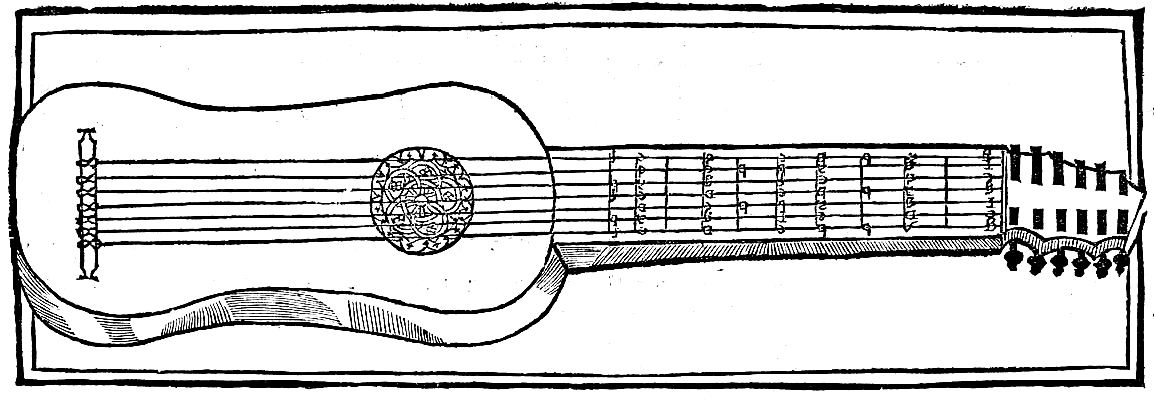
\includegraphics[width=\linewidth]{Bermudo-vihuela7}
\end{figure}
%}}}4

Indeed, vihuelas had been an important part of the Spanish royal musical ensemble
from the days of Charles I.
Vihuela intabulations survive of masses by Cristóbal de Morales and Francisco
Guerrero.%
    \Autocite[\sv{vihuela}]{Grove}
Vihuelas were almost certainly part of Cáseda's ensemble in Zaragoza, since the
instrument is mentioned frequently in the cathedral chapter acts.%
    \Autocite{Calahorra:Zaragoza2}
In Puebla, the cathedral chapter paid 100 pesos to one Diego de León in 1676
for playing the \term{vihuela de arco}, demonstrating the use of vihuelas in
the cathedral and suggesting their use as well in the closely related musical
ensemble of the Convento de la Santísima Trinidad.%
    \Autocite[44]{PerezRuiz:Aportes}

\index{Madrid!Royal Chapel}
\index{Charles I}
\index{Morales, Cristóbal de}
\index{Guerrero, Francisco}
\index{intabulation}
\index{villancico!scoring}
\index{Puebla!Convento de la Santísima Trinidad}

We know that women religious played the vihuela because one of the two
surviving vihuelas from this period, in the church of La Compañia de Jesús in
Quito, Ecuador, is believed to have been the possession of the nun Santa
Mariana de Jesús (1618--1645).
According to contemporary accounts, Mariana was especially skilled on the
instrument. 
The theological worth then attributed to the vihuela is shown in an account of
one Christmas night (probably during Matins service), when Mariana \quoted{sat
down to make music playing a vihuela, and she said that she wanted to offer
this music among the angels who were attending there}.%
\begin{Footnote}
    \Autocite[275]{EspinosaPolit:SantaMariana}, quoted in
    \Autocite[73]{Bermudez:Vihuela}.
\end{Footnote}
This form of devotional performance fits well with the original meaning of the
\foreign{kitharōdos} in \scripture{Rev 14}, \quoted{lyre-player, harpist who
plays an accompaniment to his own singing}.%
    \Autocite[\sv{kitharōdos}]{BDAG}
It is likely that the nuns of La Santísima Trinidad in Puebla also included at
least one vihuela in their musical ensemble.
It would seem strange for them not to use that instrument in performing a
villancico that used it as a metaphor for Christ (though the example of
\term{clarín} villancicos discussed in \chapref{ch:intro} suggests that an
instrument invoked symbolically need not be physically present).

\index{convent music}
\index{Quito}
\index{\emph{clarín}}

In Cáseda's villancico, the specific details of the vihuela---its construction,
tuning, playing technique, and typical stylistic idioms---provide new
allegorical possibilities for the poet to extend the cithara tradition.
More importantly, this poetic conceit of Christ as vihuela also provides Cáseda
as a composer with possibilites for actually representing the cithara symbol
through sound.
%}}}3
%}}}2

%{{{2 music
\subsection{Representing the Vihuela, Representing Christ}

In the poetry of Cáseda's villancico, the specifications of the vihuela become
symbols for Christ, particularly for his body, which suffered on the cross, was
raised, and became present to believers through the Eucharist.
The vihuela's seven strings here symbolize the seven sacraments.
According to Bermudo, the most common tuning for the seven strings was in
intervals of alternating fifths and fourths starting from a lowest string on 
\term{G (gamma, ut)}, that is, \pitch{G}{2}.%
    \Autocite[\folios{109\recto--109\verso}]{Bermudo:Declaracion}
That would make the strings \pitch{G}{2}, \pitch{D}{3}, \pitch{G}{3},
\pitch{D}{4}, \pitch{G}{4}, \pitch{D}{5}, \pitch{G}{5}.
Thus the highest and lowest strings are tuned in octaves, as copla 1 says:
\foreign{forma unida la alta con la baja}.
All the strings are tuned in perfect intervals, which may be part of the
meaning in copla 2, \foreign{en cada punto entera consonancia} (in each point
or note a whole consonance).
The \foreign{lazo} could refer either to the bow of a \term{vihuela de arco},
or to a plectrum that was sometimes used in place of the fingertips.
The poet has even incorporated the instrumental symbolism into the structure of
the verse, as the poem itself is composed primarily in lines of 7 and 11
syllables, beginning with the pattern 7--7--7--11--11---a pattern known as a
\term{lira}.%
    \Autocite{Lauer:Metrification}

\index{tuning}

Whether or not an actual vihuela was used for this villancico, Cáseda
represents the vihuela musically through the compositional structure.
First, he features the continuo section prominently, spotlighting all the
cithara-like instruments that might have been played.
The piece begins with the Tiple I (sister Tomasita in Puebla) singing a solo
against the continuo with widely-spaced open fifths and octaves between them.
The vihuela or other continuo instruments filling in the intervening space
would have stood out clearly.
Again in \measure{2}, when the Tiple I makes the striking leap up to the
B flat, she is joined only by the continuo.
In \measure{13}, there is an abrupt harmonic shift initiated by the continuo
alone, which here leads the singers rather than just accompanying them.

\index{performers!women}

Cáseda also gives the continuo several solos throughout the piece.
The first solo comes at the conclusion of the first three lines of poetry
(\measure{9}).
Surely the composer intended for more music to sound here than simply the
falling fifth of the melodic bass line.
Indeed, with the vocalists having just sung that the \quoted{divine music
\Dots{} rivals that of the birds}, it would seem natural for an instrumentalist
to fill in a little trilling bird music here.
Cáseda allows more possibilities in the coplas (\measures{52, 54, 57, 72,
76--77, 80}): in the first example, the ensemble sings \quoted{let the divine
strings resound}, and then there are two semiminims of vocal rest while the
continuo ensemble can do just that.

\index{musical topics!birdsong}

Cáseda also has the singers themselves imitate the vihuela.
In the opening gesture, the Tiple I sings her solo with continuo accompaniment,
followed by the rest of the vocal ensemble in a homorhythmic echo
(\musref{mus:CasedaJ-Que_musica_divina-opening}).
The chord voicing resembles the tuning of a vihuela, with the open fifths and
fourths in the three lower vocal parts of \measures{1--2}.
The dotted rhythm, sung all together, and the contrary motion between voices,
mimic the effect of strummed open strings on a vihuela.
The general texture of soloist against a regular rhythmic, chordal
accompaniment also evokes someone singing while playing (like Santa Mariana de
Jesús of Quito, and the \foreign{citharoedi} of \scripture{Rev 14}).
This image would be even clearer in the coplas sung by soloists with only
continuo accompaniment.

\index{musical topics!\emph{vihuela} music}
\index{imitation}

%{{{4 Caseda music opening
\begin{musicexample}
    \caption{Cáseda, \wtitle{Qúe música divina}, estribillo, opening}
    \label{mus:CasedaJ-Que_musica_divina-opening}
    \includefloat{CasedaJ-Que_musica_divina-opening}
\end{musicexample}
%}}}4

The vocal textures from \measure{6} on are more typical of vocal music,
particularly in the paired, ornament-like figures in the sections from
\measures{11--15, 19--39}.
After \measure{19}, Cáseda realizes the common villancico poetic trope of
birdsong by giving the singers birdlike trill patterns. 
At the end of the estribillo, Cáseda returns to musically representing the
vihuela/cithara trope.
In the last eight measures (\measures{47--50}), the rhythmic pattern in the
voices---a minim rest and two minims---again suggests strumming (see
\musref{mus:CasedaJ-Que_musica_divina-clausulas} below).
The estribillo ends with an alternating pattern of minor chords on G and
seventh chords over D, like the strumming of the two common vihuela chords,
known to us as \term{i} and \term{V\textsuperscript{7}}.
If this passage were played by a vihuelist in an intabulation, the player would
likely use a down-up-up strumming pattern, similar to the patterns recommended
for guitarists and harpists in Lucas Ruiz de Ribayaz's manual \wtitle{Luz y
norte musical} of 1677 (\figref{fig:Ruiz-strumming}).%
    \Autocite[9]{Ruiz:Luz}
In this rhythmic pattern, Cáseda inserts rests between syllables of the words
in this passage, and this rhetorical technique of \wtitle{tmesis} creates the
gasping effect of \quoted{dismayed}, arrested senses.

\index{Ruiz de Ribayaz, Lucas}
\index{rhetoric}

%{{{4 Ruiz strumming
\begin{figure}
    \caption{Strumming patterns in Ruiz de Ribayaz, \wtitle{Luz y norte
    musical}} 
    \label{fig:Ruiz-strumming}
    \includefloat{Ruiz-strumming}
\end{figure}
%}}}4

In the coplas, the homorhythmic, dotted opening phrase again seems to mimic
strumming.
For the phrase \foreign{forma unida la alta con la baja} (\measures{90--94}),
Cáseda sets the text on multiple levels at once.
In \measures{90--91}, the Tenor sings a pedal \pitch{D}{4}, like a droning open
string, against the Alto's moving line.
Thus the \foreign{alta} Alto is paired with the lowest voice.
The Tenor, meanwhile, forms perfect consonances (octave and fifth) with the
Bass, where a viheula on that part would likely be playing open D and G strings. 
The Tenor is thus acting like one of the strings on the vihuela.
All of these ideas are then repeated in the next phrase, \measures{92--93}, now
with G pedals, as though switching over to a different pair of strings.

These evocations of the vihuela would seem to fit with Hollander's thesis that
early modern poets shifted their interest from speculative views of music based
on ancient sources toward the details of practical contemporary music.
But in this case the tuning and performance practice of the contemporary
vihuela are harnessed as tools for theological allegory, more powerful in their
specificity than the vague term \term{cithara}.
In classic Neoplatonic fashion, the piece shows listeners how to hear
\wtitle{musica instrumentalis} while listening for the higher Music of Christ. 
The real, sounding vihuela is only a symbol of Christ.
It is Christ's musical \quoted{excellence} that is praised, not that of any
human virtuosi.

\index{Neoplatonism}
\index{\emph{musica instrumentalis}}
%}}}2

%{{{2 false music
\subsection{False Music}

\quoted{Of faith he is the intrument}, Cáseda's poem says of Christ,
\quoted{and his music regales the ear \add{or, hearing}} (copla 2).
That music, the poem says, is Christ's death on the cross.
But, as copla 5 says, \quoted{those things that his sovereign voices \add{or,
words} sound are not for the senses}.
This phrase (\foreign{no son a los sentidos}) echoes Thomas Aquinas's
description of the Eucharist: \quoted{That the true body of Christ and his
blood are in this sacrament, cannot be grasped by sensation \addorig{neque sensu}
nor by intellect, but by faith alone, which rests on divine authority}.% 
    \Autocite[question 75, article 1, \pagenum{274}]{Aquinas:Summa3}
When the villancico says, \quoted{sensation does not eat it} (\poemline{33}),
it recalls Aquinas's explanation that Christ's body is eaten in a sacramental,
not literally physical way.
Like the contests of the senses in \chapref{ch:faith-hearing}, this villancico
challenges the credibility of sensation even while appealing to it.
It prompts hearers to listen past what their ears perceive to grasp a higher
truth.
The real music of Christ's passion surpassed human understanding: in the words
of the villancico, \quoted{as many voices as the senses perceived from this
instrument will be false} or out of tune.
All this seems to be a way of saying in line with Aquinas that those who rely
on their senses, understood through reason alone, to grasp the mystery of
Christ in the Eucharist will fail.
Like Calderón's \quoted{Judaísmo} (\chapref{ch:faith-hearing}), they would be
hearing Faith without faith.

\index{Aquinas, Thomas}
\index{senses!limitations}
\index{tuning}
\index{doubt}
\index{harmony}
\index{Christ!as musician}

The reason why the music played on Christ the vihuela sounds \quoted{false} is
that in his crucifixion Christ is taking on humanity's sinful nature in order
to create harmony between humanity and God.
Here we see an intensified version of the dissonance trope in
\wtitle{Suspended, cielos} by Cererols: music that breaks earthly rules points
to \quoted{the new consonance} created by Christ.
Cáseda's villancico allows listeners to contemplate that Music, the
\quoted{mysterious excellence} or \quoted{virtuosity} of Christ the divine
musician, which \quoted{elevates to the heavens the one who reaches it}.
Since Cáseda's music with its open fifths and strumming patterns effectively
turns the whole ensemble into a vihuela, the piece becomes an active exercise
in putting the human community in tune with Christ.

Cáseda's exercises in depicting musical \quoted{falsehood} go well beyond the
mild dissonance used by Cererols, though.
In his opening (\musref{mus:CasedaJ-Que_musica_divina-opening}), Cáseda writes
direct octaves between the voice and accompaniment (in the leap up to B flat,
\measures{2}), and emphasizes them by cutting out all the other voices.
In the next two measures, Cáseda sets the word \foreign{acorde} (tuneful) to
bald parallel fifths between outer voices.
Cáseda suspends the Alto's B flat, so that these fifths move into a dissonant
seventh sonority.

These contrapuntal solecisms are what Bermudo calls musical \foreign{falsedad}.
He gives specific examples of parallel fifths and octaves, comparing them to
\quoted{barbarism in grammar}.%
    \Autocite[\folio{128\verso}]{Bermudo:Declaracion} 
In condemning this error, which he says is common for beginners and
instrumentalists, Bermudo uses some of the same key terms as Cáseda's
villancico:
\begin{quoting}
    I want to say that there are those taken for musicians who have learned
    without a teacher and with much labor, and they are poorly equipped
    \addorig{son faltos}, and they know few principles.
    This pestilence is especially great for keyboard players.  
    This is what that outstanding musician of blessed memory, Cristóbal de
    Morales, told me once, that if what many organists played would be written
    out we would find great faults.  
    And he had good reason to say it: because they can play two octaves and two
    fifths and not perceive it \add{because of the organ's timbre}: while
    singing it they would recognize the falsehood \addorig{falsedad}.% 
        \Autocite[\folio{128\verso}]{Bermudo:Declaracion} 
\end{quoting}
Direct and even parallel fifths do indeed regularly in the notated examples of
vihuela harmonization.%
    \Autocite{Araujo-Mendonca:Vihuela}
Just as in popular guitar music today, the construction of the instrument made
linear voice leading more difficult than simply shifting hand positions to
create parallel motion, and this idiom suited the chord-based music typical of
the instrument.

\index{solecisms}
\index{organ}
\index{music theory}

Cáseda has his musicians create \quoted{false} music through \quoted{dangerous}
and even intentionally erroneous counterpoint.
In the section beginning in \measure{40}, Cáseda tries out \foreign{cláusulas
varias} (various cadences), creating an effect as though all the voices are  
continually trying to cadence (\musref{mus:CasedaJ-Que_musica_divina-clausulas}).
Each of the voices sings a typical cadential pattern, but at different times
and not quite aligning relative to the others.
The chromaticism becomes more acute as the passage continues, culminating in a
bizarre collision in \measures{53--55}.
The bottom four voices here on their own in \measure{36} would appear to be
cadencing on F, with the C in the Bass to move up by fourth and the cadential E
in the Tiple II to resolve up to F.
But the top voice seems determined to cadence on G, so that in the second minim
of \measure{53} the top voice is an augmented fourth above the Bass (F sharp
against C), while the Alto's E is made to seem dissonant even when by rights it
should not be.
In \measure{54} the voices manages to cadence on D, with the top voice settling
back down to F sharp, though the Tenor has re-entered just at this point to sing
an unprepared dissonant B flat over the Bass (making an augmented fifth against
the Tiple I's F sharp).

%{{{5 Caseda clausulas
\begin{musicexample}
    \caption{Cáseda, \wtitle{Qué música divina}, \measures{40--55}:
    Conflicting \quoted{cadences} and false \term{ficta}}
    \label{mus:CasedaJ-Que_musica_divina-clausulas}
    \includefloat{CasedaJ-Que_musica_divina-clausulas}
\end{musicexample}
%}}}5

The final section of the estribillo
(\musref{mus:CasedaJ-Que_musica_divina-desmaya}) continues in this direction,
as Cáseda's music evokes the poetic idea of \quoted{elevating the senses} and
\quoted{dismaying the \add{bodily} powers}.
He begins with a wedge pattern between the Tenor and the accompaniment, again
juxtaposing B flat (in the Bass) with F sharp (in the tenor).
Cáseda brings in the next two voices, each one singing one of the two patterns
already introduced: the Alto has the ascending line, and the Tiple 2 has the
descending one.
But their entrances are flipped from that of the Bass and Tenor, so a reverse
wedge is created.
As this is happening, in \measure{61}, the Tiple I enters from out of nowhere
with a high A, skipping down to what is apparently an F natural (based on the
F sharp specified at the beginning of the next measure).
The A creates a \musFig{\na6 \fl3} sonority: on its own it is an imperfect
consonance with the Bass, but against the E flat in the Tiple II it certainly
has the effect of elevating and dismaying, amplified by the direct fifths it
then forms with the Bass as it skips down to F.
As though to ensure that listeners did not think this a mistake, Cáseda repeats
the whole passage again in \measure{67}, though with the voices rearranged.

%{{{5 Caseda desmaya
\begin{musicexample}
    \caption{Cáseda, \wtitle{Qué música divina}, \measures{63--80}: Elevating
    the senses, dismaying the faculties; rhetorical \term{tmesis} as
    strumming}
    \label{mus:CasedaJ-Que_musica_divina-desmaya}
    \includefloat{CasedaJ-Que_musica_divina-desmaya}
\end{musicexample}
%}}}5

The practice of \term{musica ficta}, still widespread in the Spanish Empire,
depended on the singer's ability to recognize places where the written pitches
needed to be inflected.%
   \Autocite{Berger:Ficta} 
As Cáseda's villancico progresses it requires more and more improvised
accidentals, until it starts to become unclear how to apply the rules, such as
in the strange collision of cadences in \measures{53--55}.
The Tiple II might begin the last phrase (starting in \measure{34} on F),
singing the E as part of a cadential formula on F and therefore natural; but
when the cadence comes on D, an E flat might be preferable. 
Either option clashes with the notated F sharp in the Tiple I.
In \measures{69--70}, on \foreign{potencias desmaya}, the ficta situation becomes
actually impossible.
To maintain the fugal motive, the Tiple II would have to sing three minim B
flats and then a semibreve B natural, leading up to C.
But in the same place as the Tiple II B flats, the Tenor has a notated sharp
sign on the B (the only way of indicating B natural in this mode).
The accidental in the Tenor part is clearly a sharp, written in the same hand
and with the same ink as the rest of the music.
This creates a cross relation---in Spanish, a \foreign{falsa relación}---between
the B flat and B natural.

\index{\emph{musica ficta}}
\index{music theory}

Any educated musicians confronted with this score would attempt to \quoted{fix}
these problems (probably by singing all B naturals in the Tiple II).
But any solution chosen feels wrong.
Is the music supposed to sound out-of-tune?
How should musicians apply ficta, how to tune intervals, when the composer is
forcing them to break the traditional rules?
The music is false: it cannot be emended with the further falsehood of musica
ficta or anything else.
That this should happen most blatantly at the opening of the piece on the very
word \foreign{acorde} is significant.
The fifths recall the tuning of the vihuela's strings, and the kind of music
typically played on the instrument. 
They were also the very paradigm of bad musicianship and untuneful composition.

Pedro Cerone specifically warned composers not to write passages that would
tempt singers to add incorrect accidentals and \quoted{falsify} the music.
Cerone uses the terms \foreign{falsa} and \foreign{falsificar} at different
times to mean either \term{musica ficta} or \quoted{wrong} notes (as in
\quoted{false relations}).
In certain situations (of which he gives a notated example, shown in
\figref{fig:Cerone-false_cadences}), \quoted{the singer can easily add a sharp to
the fifth, thinking it to be a cadence \addorig{cláusula}: for he will see that
the notes are moving in the manner of a cadence, saying \term{Sol fa sol},
\term{Re ut re}, and so on, and raising the note he will make it become false
\addorig{falsa}, and very dissonant to the ear}.% 
    \Autocite[629]{Cerone:Melopeo}
This is precisely the kind of passage Cáseda has written in his setting of
\foreign{cláusulas varias}: the parts all have typical cadential patterns like
the ones Cerone describes, and the voices would be tempted to raise certain
pitches at the wrong times. 
As with the parallel fifths that Bermudo warned against, Cáseda appears to be
breaking the rules deliberately and with symbolic intent.

\index{Cerone, Pedro}
\index{performers!applying \emph{musica ficta}}

%{{{4 cerone false cadences 
\begin{figure}
    \caption{Melodic patterns \quoted{in danger of being falsified} (sung with
    improper ficta) in Cerone, \wtitle{El melopeo y maestro}, 629} 
    \label{fig:Cerone-false_cadences}
    \includefloat{Cerone-false_cadences}
\end{figure}
%}}}4

Through his musical falsehoods, Cáseda has pushed the Neoplatonic theology of
music to the point where earthly music, rather than attempting to reflect
heavenly perfection, even if only partially, now overtly highlights its own
falsehood.
The emphasis is shifting toward using music not to reflect heaven at all, but
to aim primarily at \quoted{elevating the senses} and \quoted{dismaying the
powers}.
The goal for the hearers is moving from intellectual contemplation to affective
experience.
This change need not be seen as part of a \quoted{disenchantment} process, as
Hollander portrays it, though.
In order for Cáseda's flaunting of contrapuntal rules to have meaning, the
rules must still be preserved.
Breaking them for expressive purposes (whether affective expression or symbolic
expression, as of the Neoplatonic imperfection of \wtitle{musica
instrumentalis}) actually reflects a continued faith in the validity of those
rules.
Cáseda is not disregarding the old musical-theological system, but rather
insisting upon it so strongly that he passes over a reasonable limit and seems
to contradict himself.
As the tradition of metamusical villancicos developed, there was an increased
demand for composers both to imitate the conventions established by
predecessors and to differentiate their own works in some way. 
At the same time the concept of imitation itself, as a musical-rhetorical
practice within a Neoplatonic framework, was changing.
The three villancicos studied in this chapter demonstrate the first kind of
imitation---that of influence and homage---because they manifest a certain
degree of strain as each successive composer pushes the tradition of musical
self-representation further towards a limit of intelligibility.

\index{imitation}
\index{villancico!listener response}
\index{secularization}
\index{Hollander, John}
\index{Neoplatonism}
\index{affects}
\index{counterpoint, symbolism}

In contrast to the metamusical villancicos by Gutiérrez de Padilla and
Cererols, Bruna and Ambiela's variants of \wtitle{Suban las voces al cielo}, by
contrast, are less focused on abstract levels of music like the music of the
spheres or the angels.
Instead they use human music-making as an analogy for the dynamics of spiritual
communion, self-offering, and intercessory prayer.
The ensemble of convent sisters who sang Cáseda's villancico in Puebla embodied
through their voices the structure and style of the vihuela, a performance that
in turn interpreted that instrument as a physical sign pointing to Christ's
sufferings.
The body of Christ on the cross, made present in the Eucharist, was thus linked
to the body of the instrument, manifested symbolically through the bodies of
these women who had offered themselves in devotion to Christ.

\index{Cáseda, José de|)}
\index{musical instruments, symbolism|)}
\index{\emph{vihuela}|)}
\index{performers!women}
%}}}2
%}}}1

%{{{1 conclusions to book
\section{Conclusions}

Villancicos about music challenged composers to use the craft of music to
communicate theological ideas about music itself.
They presented hearers with the opportunity to listen for higher forms of music
through sounding music.
This complex music required that listeners be equipped with the requisite
musical, poetic, and religious knowledge and aural training to interpret it.
In line with the idea that faith was a virtue by which believers shaped
their lives in the image of Christ the Word, Catholics sought to create a
community of faithful hearers---one in which both the message and the process
of teaching were controlled under the authority of the Church.

\index{hearing}
\index{community}

This was an idealized theological vision of both the Church and of listening,
in which reliable teachers communicate without difficulty to trusting hearers,
all in perfect concord with the Holy Spirit's voice speaking down through the
hierarchy of the Christian community.
Real life was never so pristine.
Even if we could transport ourselves to Puebla Cathedral in 1657 or Lleida in
1689 we would not be able to answer the question of whether parishioners really
heard villancicos with faith---even whether they actually listened at all.
But we do know what was presented to their ears, and that is music that
directly explored the power of music to shape faith.

\index{theology!ecclesiology}
\index{audiences}

Evocations of angelic fugues and planetary cadences, castanets and vihuelas,
prompted listeners to reflect on the connections between worldly sounds and
heavenly truth.
In other words, villancicos were musical theology, sounding embodiments of a
worldview in which the Divine suffused Creation, through which God's nature
could be revealed to those who had learned to listen with faith as the book of
nature was read aloud.
If we take villancicos seriously as expressions of faith, we must conclude that
Spaniards believed music in performance could bring concord to individuals and
the community, after the pattern of the heavens.
In other words, they actively brought together Boethius's three kinds of music.
At the same time we must ask from a more mundane perspective what social
factors motivated early modern Spaniards to reiterate this theological vision
of music so vigorously.

\index{musical theology}
\index{creation}
\index{Boethius}
\index{faith}

I would argue that the notion of social harmony posed a special appeal to
people living under the Spanish crown.
The century after Columbus had transformed the complexion of the empire.
In America the minority of pure-blooded Spaniards lived under a constant threat
of native and African uprising, and the heirs of the Aztec Empire and the Kongo
Kingdom had to navigate a colonial society in which they could only be
\term{indios} and \term{negros}.
In Iberia, too, the influx of Native American goods and African slaves, not to
mention the Aztec and Inca gold underwriting the Habsburgs' growing debts,
destabilized the social order.
The theft of land and enslavement of fellow human beings put strain on Spanish
religion as well, forcing Spaniards to justify themselves.
Ethnic villancicos seem the most obvious manifestation of imperial Spain's
struggle with difference, but they are only one way that music enabled
Spaniards to make sense of this colorful and chaotic new world.
Images of human society all united in harmony, of a diversity of voices moving
together not in unison but in counterpoint, reinforced the social hierarchy in
a way that must have given comfort to the ruling class of Spain, just as it
added to the fear and confusion of their colonial subjects.%
    \Autocites
    {Baker:Harmony}
    {Irving:Colonial}
    {Illari:Polychoral}
Every clarion call reminded them that God had ordained the structures of
worldly power, just as surely as the sun was the fourth planet around a
stationary earth.
Of course, in the decades after Galileo and Newton's discoveries, people were
becoming aware that the cosmology used to justify the old regime did not square
with empirical observation; but in Spain the response was to insist all the
more strongly on the beauty of the old worldview.
Even as Spaniards began to emphasize the imperfection of music and creation
toward the end of the seventeenth century, they still did so as part of a 
Neoplatonic conception.

\index{harmony!social}
\index{Native Americans}
\index{Africans}
\index{slavery}
\index{villancicos!ethnic}
\index{\emph{clarín}}
\index{Galilei, Galileo}
\index{Newton, Isaac}
\index{science}
\index{perfection}
\index{Neoplatonism}
\index{villancico!social functions!project political power}
\index{colonialism}
\index{cosmos}

At the same time, though, the villancicos we have studied do not all present a
simple picture of social conformity.
From the worldly thrill of \term{jácara} outlaw ballads to the expressions of
doubt and misunderstanding in the dialogues of the deaf, villancicos did invite
a degree of critical reflection on the Church's role in contemporary society.
They were not just impositions of dogma or diverting but meaningless doggerel.
They asked hearers to doubt their own experiences and to temper their sensation
with faith.
They asked people to listen with faith, for faith.
And through their appeals both to social cohesion and to personal affective
response and commitment, they exhorted people to move past simple belief into
lives of faithfulness.

\index{villancico!listener response}
\index{doubt}
\index{hearing!training}
\index{\emph{jácara}}
\index{deafness}

Still, given the depths of injustice and hypocrisy in the Spanish Church during
the era of slavery and colonialism, it is not hard to understand the critique
of Juan de la Cruz (\chapref{ch:faith-hearing}) that Spaniards had their ears so
full of sweet harmonies that they were deaf to the actual call of Christ.%
    \Autocite
    [\range{bk}{3}, \range{ch}{45}, \pagenum{425}]
    {JuandelaCruz:Subida}
Music could help faith come through hearing, but as the friar Antonio de
Azevedo warned, what was heard had to come from \quoted{the word of Christ},
and people needed to be equipped to understand and receive it.%
    \Autocite{Azevedo:Catecismo}
Otherwise \quoted{all is vanity and a chasing after wind}
(\scripture{Eccl 1:14}).
All the harps and shawms and polychoral counterpoint in imperial Spain
amounted to no more than \quoted{noisy gongs and clanging cymbals}
(\scripture{1Cor 13:1}) if they did convert hearers of the word into doers
(\scripture{Jas 1:22}).

\index{Juan de la Cruz}
\index{Azevedo, Antonio de}
\index{faithfulness}
\index{villancico!ethical value}
\index{theology!ethical}
%}}}1

